\chapter{Results}


Analyzing the results obtained with the original parameters from 
the article by Parham and Michael 
($T' = 19.9 \ (\text{also called $T_1$ in the article}), \ T_1=23.2, \ T_2=0.07, \ \omega_1=0.67, \ \phi_1=1.53, \ R_1=85.9, \ R_2=0.98, 
\ \omega_2=0.65, \ \phi_2=1.99, \ A=-0.03, \ B=1.31, \ C=-4.4, \ b_1=0.04, \ 
b_2 = 0.09, \ T_{min}=14.5, \ \gamma= 1/120, \ R_L = 50, \ c_1=0.00554, \ 
c_2=-0.06737$ \cite{Parham2010}, \cite{OKUNEYE201772}), and using 
the previously estimated average population and an arbitrary value 
for the mosquito population, of 10000, assuming 1000 infected humans and 
5000 exposed mosquitoes at $t=0$, the modeling is as follows
\footnote{The development of the model with the original data can be found at 
https://github.com/RaphaLevy/Undergraduate\_Dissertation/blob/main/
\\modeling\_files/Original\_Parameters.ipynb.}: 

% Pra plotar duas imagens uma ao lado da outra, precisa corrigir a posição das legendas.

% \begin{figure}
% \hspace*{-1.5cm} % Adiciona espaço negativo para puxar a imagem para a esquerda
% \begin{minipage}{.45\textwidth}
%   \centering
%   \includegraphics[width=1.25\linewidth]{SIR_Dados_Originais_Parham_Michael.png}
%   \captionof{figure}{A figure}
%   \label{fig:test1}
% \end{minipage}%
% \hspace{1.5cm} % Adiciona espaço horizontal
% \begin{minipage}{.45\textwidth}
%   \centering
%   \includegraphics[width=1.3\linewidth]{SEI_Dados_Originais_Parham_Michael.png}
%   \captionof{figure}{Another figure} % Legenda à direita da segunda imagem
%   \label{fig:test2}
% \end{minipage}
% \end{figure}





\begin{figure}[!ht]
        \centering
        \hbox{\hspace{6em} 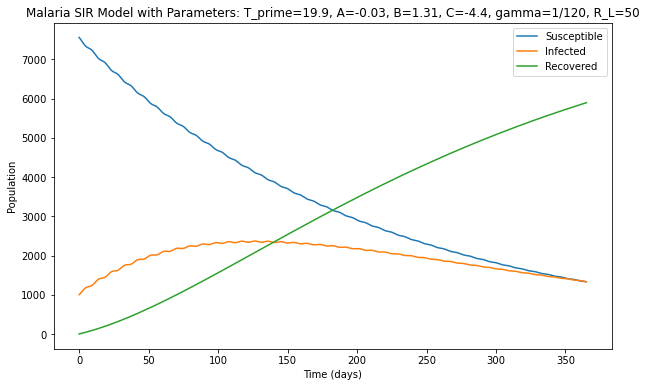
\includegraphics[scale=0.45] {THESIS-SIR_Dados_Originais_Parham_Michael_CORRECAO.png}}
        \caption{SIR with original parameters}
\end{figure} 
\begin{figure}[!ht]
        \centering
        \hbox{\hspace{6em} 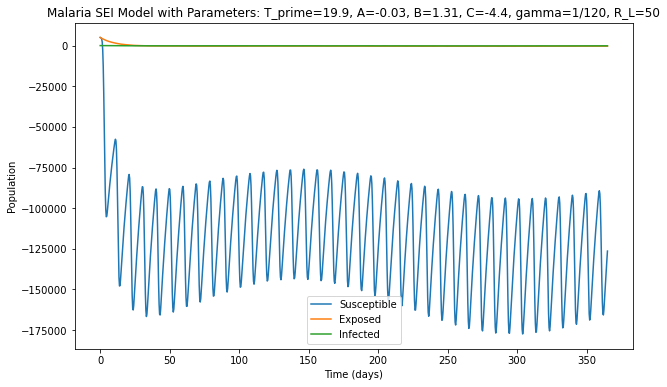
\includegraphics[scale=0.45] {THESIS-SEI_Dados_Originais_Parham_Michael_CORRECAO.png}}
        \caption{SEI with original parameters}
\end{figure} 
\newpage
With this initial modeling, 
a strong oscillation in the number 
of susceptible humans and mosquitoes, 
as well as infected humans, is noticeable. 
Furthermore, it is evident that with these 
parameters, the disease will not become endemic, 
as the number of infected humans tends to 0 
throughout the year, while the population of 
susceptible mosquitoes becomes negative, and the 
population of exposed and infected individuals also tends to 0. 
These effects were characterized by temperature and 
precipitation oscillating in very short periods of 
time, attributed to a high value of $\omega$ for both functions.
\\\\
Starting with only a single infected human and exposed mosquito, the 
oscilatting population isn't noticeable in the SIR plot, however the mosquito population 
still becomes negative.
\\\\
Now, the first necessary modification is to correct the temperature 
and precipitation to consider data from Manaus, as the original 
paper uses data from Tanzania. So, 
collecting climatological data from Manaus from \cite{ClimaMANAUS}, 
the average temperature and precipitation were estimated 
as 26.4 $^\circ C$ and 250.083 mm, respectively. 
With this data, the amplitude of seasonal variability, 
angular frequency, and phase lag of variability for 
both were defined to approximate the real values:
\\\\
\begin{adjustwidth}{-0.5cm}{}
\begin{center}
\renewcommand{\arraystretch}{1.5}
\begin{tabular}{|c | c|} 
 \hline
 \textbf{Parameter} & \textbf{Value}\\ 
 \hline
  $T_1$ & \makecell[l]{\rule{0pt}{3ex}26.4$^\circ C$\rule[-1.5ex]{0pt}{0pt}} \\
 \hline
 $T_2$ & \makecell[l]{\rule{0pt}{3ex}0.025\rule[-1.5ex]{0pt}{0pt}} \\
 \hline
 $\omega_1$ & \makecell[l]{\rule{0pt}{3ex}0.017 (months)$^{-1}$\rule[-1.5ex]{0pt}{0pt}} \\
 \hline
 $\phi_1$ & \makecell[l]{\rule{0pt}{3ex}-1.45\rule[-1.5ex]{0pt}{0pt}} \\
 \hline
 $R_1$ & \makecell[l]{\rule{0pt}{3ex}250.083 mm\rule[-1.5ex]{0pt}{0pt}} \\
 \hline
 $R_2$ & \makecell[l]{\rule{0pt}{3ex}0.565\rule[-1.5ex]{0pt}{0pt}} \\
 \hline
 $\omega_2$ & \makecell[l]{\rule{0pt}{3ex}0.02 (months)$^{-1}$\rule[-1.5ex]{0pt}{0pt}} \\
 \hline
 $\phi_2$ & \makecell[l]{\rule{0pt}{3ex}1.6\rule[-1.5ex]{0pt}{0pt}} \\
 \hline
\end{tabular}
\captionof{table}{Values for climatic parameters}
\end{center}
\end{adjustwidth}

\vspace{1cm}
The amplitude parameters ($T_2$ and $R_2$) and phase lag 
parameters ($\phi_1$ and $\phi_2$) are dimensionless. 
The temperature and precipitation throughout the year 
then evolve as follows
\footnote{The development of the model with the original data can be found at 
https://github.com/RaphaLevy/Undergraduate\_Dissertation/blob/main/
\\modeling\_files/Adapting\_T\_and\_R.ipynb.}:

% \begin{figure}
% \hspace*{-1.5cm} % Adiciona espaço negativo para puxar a imagem para a esquerda
% \begin{minipage}{.45\textwidth}
%   \centering
%   \includegraphics[width=1.2\linewidth]{Grafico_da_Temperatura.png}
%   \captionof{figure}{A figure}
%   \label{fig:test1}
% \end{minipage}%
% \hspace{1.5cm} % Adiciona espaço horizontal
% \begin{minipage}{.45\textwidth}
%   \centering
%   \includegraphics[width=1.2\linewidth]{Grafico_da_Precipitacao.png}
%   \captionof{figure}{Another figure} % Legenda à direita da segunda imagem
%   \label{fig:test2}
% \end{minipage}
% \end{figure}


\begin{figure}[!ht]
        \centering
        \hbox{\hspace{6.0em} 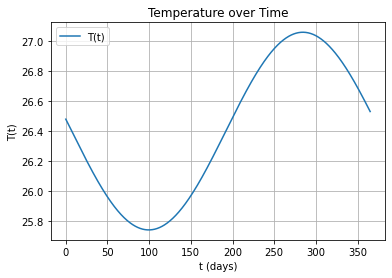
\includegraphics[scale=0.7] {THESIS-Grafico_da_Temperatura.png}}
        \caption{Temperature graph}
\end{figure} 
\begin{figure}[!ht]
        \centering
        \hbox{\hspace{6.5em} 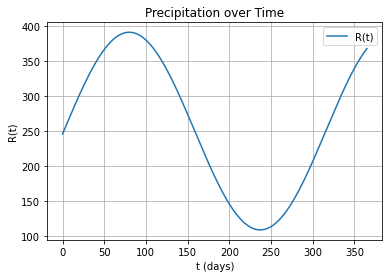
\includegraphics[scale=0.7] {THESIS-Grafico_da_Precipitacao.png}}
        \caption{Precipitation graph}
\end{figure} 
In order to ensure the correctness of the function 
with the parameters used, I calculated the temperature 
values for the months of October and May, which are the 
hottest and coldest months of the year with average 
temperatures of 27.6 $^\circ C$ and 25.8 $^\circ C$, respectively. 
Additionally, I calculated the precipitation values in March 
and August, which are the months with the highest and lowest 
precipitation, with 395 mm and 114 mm, respectively. 
The obtained average values were 27.06 $^\circ C$, 25.86 $^\circ C$, 
390.67 mm, and 112.89 mm. 
\\\\With the temperature and precipitation parameters ready for an 
initial analysis, the evolution of human and mosquito populations 
was verified.  
The results can be found in Appendices 1 and 2 
\footnote{The development of the graphs above can be found at 
https://github.com/RaphaLevy/Undergraduate\_Dissertation/blob/main/
\\modeling\_files/Adapting\_T\_and\_R.ipynb.}. 
\\\\
Notably, this result is still incorrect, as the mosquito population
still becomes negative over time. 
However, the daily oscillations
was indeed eliminated, due to the modifications made to $\omega_1$ and $\omega_2$.
Another parameter that should also be adapated in consideration for our new climatic
values was $R_L$, the rainfall limit beyond which breeding sites get flushed out and no 
immature stages survive. In the original paper, $R_L$ was defined as 50 mm, which is
too low for the high precipitation in the Amazon, which has a maximum of almost
400 mm in March. Because of this, I increased $R_L$ from 50 mm to 450 mm.
The results can be found in Appendices 3 and 4 
\footnote{The development of the graphs above can be found at 
https://github.com/RaphaLevy/Undergraduate\_Dissertation/blob/main/
\\modeling\_files/Adapting\_T\_and\_R.ipynb.}.
\\\\
Now, while the mosquito population in non-negative, it rapidly declines and
becomes extinct. That is due to the value of $\mu$, the mortality rate of mosquitoes,
given by $-\log(e^{(-1 / (AT^2 + BT + C))})$. For small values of 
$A$, $B$ and $C$, mostly $A$, $\mu$ becomes ``relatively'' large, and the mosquito
population goes extinct. To fix this, I altered these 3 parameters from the initial values 
of the arcticle, which had $\mu \approx 0.0027$, to $A=356.3, \ B=15$
and $C=-48.78$, which gave a $\mu$ of approximately $4.02133 \times 10^{-6}$, 
and so the mosquto population is nearly constant throughout the analysis.
The results, with $A, \ B$
and $C$ as above, can be found in Appendices 5 and 6 
\footnote{The development of the graphs above can be found at 
https://github.com/RaphaLevy/Undergraduate\_Dissertation/blob/main/
\\modeling\_files/Modifying\_Constant\_Parameters.ipynb.}.
\\\\
Now, it is possible to see that the mosquito population in fact remains nearly constant,
as there is close to no transference between compartments.
\\\\
To verify what else could be done to allow the 
transference of individuals between compartments,
given the differential equations of the SEI model and the 
parameters provided to achieve this goal, the value of $\mu$ becomes 
very close to 0, as seen above, while $l(\tau_M)$, a probability, becomes very 
close to 1. Therefore, $\dfrac{dE_M}{dt}$ also becomes very close to 0, 
causing the exposed function to be linear, while the mosquito population 
leaving the susceptible compartment almost simultaneously enters 
the infected compartment, causing mirrored oscillations of $S$ and $I$. 
To overcome this effect, it was necessary to modify the use of $b_1$ to 
only move mosquitoes from compartment $S$ to $E$, requiring the inclusion 
of a new parameter, $b_3$, to move mosquitoes from compartment $E$ to $I$. 
This rate is inversely related to the incubation period, so we define
\begin{gather*}
b_3 = \dfrac{T-T_{min}}{DD}
\end{gather*}
Moreover, the parameter $a(T)$ in the transition from 
exposed mosquitoes to infected was removed, as no new bites occur 
in this change from compartment $E$ to $I$.
\\\\
With these modifications, the differential equations of the SEI model were modified:
\begin{gather*}
\begin{cases}
\dfrac{dS_M}{dt} = b - ab_1\bigg(\dfrac{I_H}{N}\bigg)S_M - \mu S_M\\
\\
\dfrac{dE_M}{dt} = ab_1\bigg(\dfrac{I_H}{N}\bigg)S_M - \mu E_M - b_3E_Ml\\
\\
\dfrac{dI_M}{dt} = b_3E_Ml -\mu I_M\\
\end{cases}
\end{gather*}
\\\\
The results can be seen in Apendices 7 to 10, using $T'=19.9^\circ C$, as originally used,
and $T'=24.4^\circ C$, which is a value lower than the minimum temperature, close to $25.6^\circ C$.
Using $T'=19.9^\circ C$, the human population remains close to what could be seen in Appendix 5,
while the mosquito population is now oscillating, with the number of exposed 
mosquitoes decreasing to values near 0, while the infected population increases.
With $T'=24.4^\circ C$, the SEI plot is very similar, however the increase 
of the infected population is less noticeable.
In the case of the human population, it can be seen that the disease begins 
at a later time, and the maximum number of infected individuals is lower than
what was seen before
\footnote{The development of the graphs above can be found at 
https://github.com/RaphaLevy/Undergraduate\_Dissertation/blob/main/
\\modeling\_files/SEI\_Exposed\_to\_Infected.ipynb.}.
\\\\
Another necessary modification was to disassociate $l$, the probability of mosquito 
survival during the sporozoite cycle, from the infection rate of exposed individuals $b_3$.
\begin{gather*}
        \begin{cases}
        \dfrac{dS_M}{dt} = b - ab_1\bigg(\dfrac{I_H}{N}\bigg)S_M - \mu S_M\\
        \\
        \dfrac{dE_M}{dt} = ab_1\bigg(\dfrac{I_H}{N}\bigg)S_M - \mu E_M - b_3E_M -lE_M\\
        \\
        \dfrac{dI_M}{dt} = b_3E_M -\mu I_M\\
        \end{cases}
        \end{gather*}
With this alteration, it was noted that both populations didn't reach an equilibrium
in the first year of analysis, so extending it to 5 years, the results were as seen in Appendices 11 to 14 
\footnote{The development of the graphs above can be found at 
https://github.com/RaphaLevy/Undergraduate\_Dissertation/blob/main/
\\modeling\_files/SEI\_Exposed\_to\_Infected.ipynb.}. 
\\\\
With the SIR/SEI model now properly corrected, it was possible 
to proceed with the analyses of deforestation application. 
To do so, I began by calculating the $\mathcal{R}_0$ for both SIR and SEI, 
as well as for the coupled model, using the formulation from 
P. van den Driessche \cite{VANDENDRIESSCHE200229} as a reference:
\\\\
Firstly, we define $X_s$ as the set of all disease-free states, 
$$X_s=\{x \geq 0|x_i=0, i=1,\ldots,m\},$$
where $X=(x_1,\ldots, x_n)^T$, such that $x_i\geq 0$ represents the number 
of individuals in each compartment, and we assume each function to be 
continuously differentiable at least twice in each variable ($C^2$).
\\\\
Now, we rearrange the equations so that the first $m$ equations 
contain the infected individuals. Let ${\mathcal F}_i(x)$ be the 
rate of appearance of new infections in compartment $i$, 
${\mathcal V}_i^+(x)$ be the rate of individuals entering 
compartment $i$ by other means, and ${\mathcal V}_i^-(x)$ 
be the rate of individuals leaving compartment $i$. The disease 
transmission model consists of non-negative initial conditions 
together with the following system of equations:
$$\dot{x}=f_i(x)={\mathcal F}_i(x)-{\mathcal V}_i(x), i=1,\ldots, n,$$
where ${\mathcal V}_i (x) = {\mathcal V}_i^{-}(x) - {\mathcal V}_i^+(x)$. 
We also define 
$F=\left[\frac{\partial {\mathcal F}_i (x_0)}{\partial x_j}\right]$ 
and $V=\left[\frac{\partial {\mathcal V}_i (x_0) }{\partial x_j}\right]$, 
where $x_0$ is a Disease-Free Equilibrium (DFE), and $1\leq i,j \leq m$.
\\\\
This is equivalent to the Jacobian of these two matrices, 
after substituting $x_0$, i.e., $S=1$. $\mathcal{R}_0$ will be given 
by $\rho(FV^{-1})$, in other words, it will be the spectral radius 
of the matrix $FV^{-1}$. With the necessary definitions, we can 
calculate the $\mathcal{R}_0$ for both models as follows:
\begin{itemize}
\item \textbf{SIR:}
In this case, $m=1$, and our compartments will be arranged as $[I_H, S_H, R_H]$. Since $\mathcal{R}_0$ is calculated with normalized values, we will multiply the necessary equations by $N$ to remove the denominator. Specifically, for the SIR case, as $R_H$ is not used in any of the equations, we can express it solely in terms of $S$ and $I$. Therefore:
$$ {\mathcal F}_i(x): \text{ rate of appearance of new infected individuals in compartment } i $$
$$ {\mathcal F} =\begin{bmatrix}
a  b_2  I_M  S_H \\
\end{bmatrix} $$
Additionally, we have
$$ {\mathcal V}_i(x)^-: \text{ rate of leaving compartment } i $$
$$ {\mathcal V}_i(x)^+: \text{ rate of entering compartment } i $$
Thus:
$$
{\mathcal V^-} = \begin{bmatrix}
\gamma I_H\\
\end{bmatrix}
$$
$$
{\mathcal V^+} = \begin{bmatrix}
0\\
\end{bmatrix}
$$
$${\mathcal V}_i (x) = {\mathcal V}_i(x)^{-} - {\mathcal V}_i(x)^+$$
Therefore,
$$
{\mathcal V} =
\begin{bmatrix}
\gamma I_H\\
\end{bmatrix}
$$
\\
Hence
$$ F = \dfrac{\partial{\mathcal F}}{\partial I_M} =\begin{bmatrix}
a  b_2  S_H \\
\end{bmatrix} $$
$$ V = \dfrac{\partial{\mathcal V}}{\partial I_H} =\begin{bmatrix}
\gamma \\
\end{bmatrix} $$
\\At the equilibrium, $[S_H^*, I_H^*] = [1,0]$, so $F=[a  b_2], \ V = [\gamma]$ and $\mathcal{R}_0 = \Big | \dfrac{ab_2}{\gamma}\Big | $.

\item \textbf{SEI:}
In this case, $m=2$, and our compartments will be arranged as $[E_M, I_M, S_M]$. Again, we multiply the necessary equations by $N$ to remove the denominator. Therefore:
$$ {\mathcal F} =\begin{bmatrix}
a b_1 I_H S_M\\
0\\
\end{bmatrix} $$
$$
{\mathcal V^-} = \begin{bmatrix}
E_M (\mu + b_3 + l)\\
\mu I_M
\end{bmatrix}
$$
$$
{\mathcal V^+} = \begin{bmatrix}
0\\
b_3 E_M\\
\end{bmatrix}
$$
$${\mathcal V}_i (x) = {\mathcal V}_i(x)^{-} - {\mathcal V}_i(x)^+$$
Thus,
$$
{\mathcal V} =
\begin{bmatrix}
E_M (\mu + b_3 + l)\\
\mu I_M - b_3 E_M\\
\end{bmatrix}
$$
\\
Hence
$$ F = \dfrac{\partial{\mathcal F}}{\partial E_M, I_H} =\begin{bmatrix}
\dfrac{\partial ab_1 I_H S_M}{\partial E_M} & \dfrac{\partial ab_1 I_H S_M}{\partial I_H}\\
\dfrac{\partial 0}{\partial E_M} & \dfrac{\partial 0}{\partial I_H}\\
\end{bmatrix} = 
\begin{bmatrix}
0 & ab_1 S_M\\
0 & 0\\
\end{bmatrix}$$
$$ V = \dfrac{\partial{\mathcal V}}{\partial E_M, I_M} =\begin{bmatrix}
\dfrac{\partial E_M (\mu + b_3 + l)}{\partial E_M} & \dfrac{\partial E_M (\mu + b_3 + l)}{\partial I_M}\\
\dfrac{\partial \mu I_M - b_3 E_M}{\partial E_M} & \dfrac{\partial \mu I_M - b_3 E_M}{\partial I_M}\\
\end{bmatrix} = 
\begin{bmatrix}
\mu+b_3+l & 0\\
- b_3 & \mu\\
\end{bmatrix}$$
\\At the equilibrium, $[S_M^*, E_M^*, I_M^*] = [1,0,0]$, so $$F=\begin{bmatrix}
0 & ab_1\\
0 & 0\\
\end{bmatrix},$$
$$V = \begin{bmatrix}
\mu+b_3+l & 0\\
- b_3 & \mu\\
\end{bmatrix}$$ and $\mathcal{R}_0 = \Big | \dfrac{ab_1b_3}{(b_3+l+\mu)\mu}\Big | $.

\item \textbf{SIR/SEI:}
In this case, $m=3$, and our compartments will be arranged as $[I_H, E_M, I_M, S_H, S_M]$. Once again, we multiply the necessary equations by $N$ to remove the denominator. Therefore:
$$ {\mathcal F} =\begin{bmatrix}
a  b_2  I_M  S_H \\
a b_1 I_H S_M\\
0\\
\end{bmatrix} $$
$$
{\mathcal V^-} = \begin{bmatrix}
\gamma I_H\\
E_M (\mu + b_3 + l)\\
\mu I_M
\end{bmatrix}
$$
$$
{\mathcal V^+} = \begin{bmatrix}
0\\
0\\
b_3 E_M \\
\end{bmatrix}
$$
$${\mathcal V}_i (x) = {\mathcal V}_i(x)^{-} - {\mathcal V}_i(x)^+$$
Thus,
$$
{\mathcal V} =
\begin{bmatrix}
I_H \gamma \\
E_M (\mu + b_3 + l)\\
\mu I_M - b_3 E_M\\
\end{bmatrix}
$$
\\
Hence
$$ F = \dfrac{\partial{\mathcal F}}{\partial I_H, E_M, I_M} =\begin{bmatrix}
\dfrac{\partial ab_2 I_M S_H}{\partial I_H} & \dfrac{\partial ab_2 I_M S_H}{\partial E_M} & \dfrac{\partial ab_2 I_M S_H}{\partial I_M}\\
\dfrac{\partial ab_1 I_H S_M}{\partial I_H} & \dfrac{\partial ab_1 I_H S_M}{\partial E_M} & \dfrac{\partial ab_1 I_H S_M}{\partial I_M}\\
\dfrac{\partial 0}{\partial I_H} & \dfrac{\partial 0}{\partial E_M} & \dfrac{\partial 0}{\partial I_M}\\
\end{bmatrix} = 
\begin{bmatrix}
0 & 0 & ab_2 S_H\\
ab_1 S_M & 0 & 0\\
0 & 0 & 0
\end{bmatrix}$$
$$ V = \dfrac{\partial{\mathcal V}}{\partial I_H, E_M, I_M} =\begin{bmatrix}
\dfrac{\partial \gamma I_H}{\partial I_H} & \dfrac{\partial \gamma I_H}{\partial E_M} & \dfrac{\partial \gamma I_H}{\partial I_M}\\
\dfrac{\partial E_M (\mu + b_3 + l)}{\partial I_H} & \dfrac{\partial E_M (\mu + b_3 + l)}{\partial E_M} & \dfrac{\partial E_M (\mu + b_3 + l)}{\partial I_M}\\
\dfrac{\partial \mu I_M - b_3 E_M}{\partial I_H} & \dfrac{\partial \mu I_M - b_3 E_M}{\partial E_M} & \dfrac{\partial \mu I_M - b_3 E_M}{\partial I_M}\\
\end{bmatrix} = 
$$
$$
\begin{bmatrix}
\gamma & 0 & 0\\
0 & b_3+l+\mu & 0\\
0 & -b_3 & \mu
\end{bmatrix}$$
\\At the equilibrium, $[S_H^*, S_M^*, I_H^*, E_M^*, I_M^*] = [1,1,0,0,0]$, so $$F=\begin{bmatrix}
0 & 0 & ab_2\\
ab_1 & 0 & 0\\
0 & 0 & 0
\end{bmatrix},$$
$$V = \begin{bmatrix}
\gamma & 0 & 0\\
0 & b_3+l+\mu & 0\\
0 & -b_3 & \mu
\end{bmatrix}$$ 
and $\mathcal{R}_0 = \Big | \sqrt{\dfrac{a^2 b_1 b_2 b_3}{(b_3 + l + \mu)\gamma \mu}}\Big | = 
\sqrt{\mathcal{R}_{0 SIR} \times \mathcal{R}_{0 SEI}}$. 
\end{itemize}
We can verify that $\mathcal{R}_0$ is indeed dimensionless: 
$a, \ b_3, \ l, \ \mu$, and $\gamma$ are functions with units 
of 1/day, while $b_1$ and $b_2$ are dimensionless. Therefore, 
$\mathcal{R}_0$ for the SIR model has dimensions of (1/day)/(1/day), 
$\mathcal{R}_0$ for the SEI model has dimensions of (1/day$^2$)/(1/day$^2$), 
and the coupled model has dimensions of (1/day$^3$)/(1/day$^3$).
\\\\
Before continuing with the modeling, it was decided to analyze the evolution
of the rates as a function of temperature and precipitation, instead of time,
to see their behavior as $T$ and $R$ vary. In this case, $T'$ was used 
with value $25.6^{\circ}C$, in order to approximate
$\mathcal{R}_0$ to 0.5, which will be used later in the dissertation. 
The results can be found starting on
Appendix 15 
\footnote{The development of the graphs above can be found at 
https://github.com/RaphaLevy/Undergraduate\_Dissertation/blob/main/
\\modeling\_files/Plotting\_Rates.ipynb.}.
\\\\
Tendo obtido a fórmula fechada de $\mathcal{R}_0$, foi possível calcular o seu valor para o 
modelo atual, apresentado nos apêndices 13 e 14. No caso, $\mathcal{R}_0$ = 88.16804666190774
e a taxa de picadas no tempo $t=0$ foi de 0.025218306088151666, ou seja, aproximadamente 
uma picada por mosquito a cada 40 dias. Notavelmente, esses são valores muito altos para 
o número de reprodução de uma doença, nesse caso indicando que um indíviduo poderia infectar 
outros 88. Sendo assim, seria necessário modificar os parâmetros para que o valor de 
$\mathcal{R}_0$ ficasse próximo de 1, para que seja mais fácil analisar como pequenas 
modificações nos parâmetros causariam a extinção ou a continuação da doença. 
Antes disso, porém, 
foi necessário mais uma vez corrigir as equações do SEI, já que a probabilidade diária de 
sobrevivência de mosquitos durante o ciclo de esporozoitos ($l$), não é diretamente associada 
à taxa de infecção dos expostos, e também não é parte da taxa de entrada de novos indíviduos 
no compartimento $I$. Outra coisa que teve de ser corrigida foi a fórmula da taxa de picadas 
($a$), que voltou a ser $\dfrac{(T(t) - T')}{D_1}$ como originalmente. As equações corrigidas 
do SEI ficaram como a seguir:
\begin{gather*}
\begin{cases}
\dfrac{dS_M}{dt} = b - ab_1\bigg(\dfrac{I_H}{N}\bigg)S_M - \mu S_M\\
\\
\dfrac{dE_M}{dt} = ab_1\bigg(\dfrac{I_H}{N}\bigg)S_M - \mu E_M - b_3E_M -lE_M\\
\\
\dfrac{dI_M}{dt} = b_3E_M -\mu I_M\\
\end{cases}
\end{gather*}
Tendo corrigido as equações, o $\mathcal{R}_0$ do SEI e 
do modelo acoplado foram 
$\Big | \dfrac{ab_1b_3}{(b_3+l+\mu)\mu}\Big | $ 
e $\Big | \sqrt{\dfrac{a^2b_1b_2b_3}{(b_3+l+\mu)\gamma\mu}}\Big | $, 
respectivamente. 
Podemos verificar que $\mathcal{R}_0$ é de fato 
adimensional: $a, \ b_3, \ l, \ \mu$ e $\gamma$ são funções de 
unidade 1/dia, enquanto $b_1$ e $b_2$ são adimensionais. 
Sendo assim, $\mathcal{R}_0$ do SIR tem dimensão (1/dia)/(1/dia), 
$\mathcal{R}_0$ do SEI tem dimensão (1/dia$^2$)/(1/dia$^2$) e o 
acoplado tem dimensão (1/dia$^3$)/(1/dia$^3$). 
\\\\
Novamente calculando o $\mathcal{R}_0$ do modelo atual, seu valor para o modelo acoplado 
foi de 63.745319442750855, o que já é menor que o encontrado previamente, mas ainda muito alto. 
Foi necessário analisar que parâmetros poderiam ser modificados de forma que $\mathcal{R}_0$ 
se aproximasse de 1 tanto para o SIR quanto para o SEI, já que pelas equações é possível 
aproximar o valor acoplado de 1 enquanto que o valor de um dos outros dois modelos fosse 
menor que 1, fazendo com que a doença não se estabilizasse ou a população tendesse à extinção, 
no caso do SEI.
\\
Dessa maneira, as modificações ideais para aproximar $\mathcal{R}_0$ de 1 foram as seguintes:
\begin{flalign*}
& T' = 27.4 \Rightarrow 25.6 \\
& D_1 = 36.5 \Rightarrow 55 \\
& A = 317.925 \Rightarrow 15 \\
& b_2 = 0.3 \Rightarrow 0.2 \\
& \gamma = 1/1825 \Rightarrow 1/365
\end{flalign*}
Com essas adaptações, 
\begin{flalign*}
& \mathcal{R}_0 \ \text{SIR} = 1.167378607783994 \\
& \mathcal{R}_0 \ \text{SEI} = 1.7805860145371295 \\
& \mathcal{R}_0 \ \text{SIR/SEI} = 1.4417413161486372
\end{flalign*}
\begin{figure}[!ht]
        \centering
        \hbox{\hspace{3.5em} \includegraphics[scale=0.6] {SIR_R0_near1.png}}
        \caption{SIR com $T'=25.6 ^\circ C, \ A=15 \ (^\circ C^2 \ \text{dias})^{-1}, \ D_1=55 \ (^\circ C \ \text{dias}), \ b_2=0.2, \ \gamma=1/365$}
\end{figure} 
\begin{figure}[!ht]
        \centering
        \hbox{\hspace{3.5em} \includegraphics[scale=0.6] {SEI_R0_near1.png}}
        \caption{SEI com $T'=25.6 ^\circ C, \ A=15 \ (^\circ C^2 \ \text{dias})^{-1}, \ D_1=55 \ (^\circ C \ \text{dias}), \ b_2=0.2, \ \gamma=1/365$}
\end{figure}
\\\\
Discutindo essa aproximação de $\mathcal{R}_0$ a 1 com o orientador do 
Trabalho, foi decidido 
que ao invés de aumentar o valor $D_1$, um parâmetro empírico usado para 
estabilizar a taxa de picadas, seria ideal modificar $b_1$ e $b_2$, que são as
proporções de picadas gerando infecção em mosquitos e humanos suscetíveis, 
respectivamente, tendo em vista que, conforme temos mais ocorrências de áreas 
desmatadas, haverá um maior contato entre humanos e mosquitos, aumentando a 
proporção de picadas gerando infecção. 
\\\\
Junto com essa correção, também 
foram modelados os gráficos de evolução das taxas utilizadas, em função 
da temperatura e precipitação, ao invés do tempo, para que fosse 
possível analisar o comportamento dessas taxas conforme a temperatura e 
precipitação variam. Os gráficos estão indicados no apêndice, partindo do 15. 
Gerando esses gráficos, também foi percebido que seria ideal aumentar $R_L$ 
do valor atual de 312 mm para 450 mm, para evitar que a probabilidade de 
sobrevivência de mosquitos durante as diferentes fases se 
tornasse muito próximo de 0, o que estava afetando a taxa de 
nascimentos $b(R,T)$, e diminuir $\gamma$ de 1/365 dias para 1/120, valor original
do artigo de referência \cite{Parham2010}, de forma que a curva epidêmica fosse mais
próxima do analisado na realidade, visto na Figura 5 que a curva de infectados começa
a crescer logo no início da análise, e a infecção só deixa de ocorrer após mais de
5 anos.
\\\\
Após o desenvolvimento dos gráficos das taxas, foi iniciada a modelagem usando os dados 
``reais" da população obtidos através da interpolação dos dados de população de Manaus indicada na Tabela 4.
Com os valores previmente obtidos, a taxa anual de nascimentos foi estimada como sendo de 206.8 
nascimentos por ano. Sendo assim, são 0.56657 nascimentos por dia, aproximadamente, e 0.00007 nascimentos
diários por pessoa, já que a população rural média em Manaus é de aproximadamente 8078.5 pessoas entre 2004 e 2008.
\\\\
Assumindo que a taxa de natalidade e mortalidade de humanos é a mesma, foi então incluído na 
modelagem o parâmetro $\mu_H$, com valor 0.00007, representando a taxa diária de 
nascimentos e mortes. O modelo atualizado ficou como a seguir:
\begin{gather*}
\begin{cases}
\dfrac{dS_H}{dt} = \mu_HN-ab_2\bigg(\dfrac{I_M}{N}\bigg)S_H - \mu_HS_H\\
\\
\dfrac{dI_H}{dt} = ab_2\bigg(\dfrac{I_M}{N}\bigg)S_H-\gamma I_H - \mu_HI_H\\
\\
\dfrac{dR_H}{dt} = \gamma I_H - \mu_HR_H\\
\\
\end{cases}
\end{gather*}
A elaboração dos gráficos, a partir do Apêndice 27, foi feita em \footnote{https://github.com/RaphaLevy/TCC/blob/main/Modelagem\_com\_Dinamica\_Pop/ \\
Modelagem\_com\_Entrada\_Populacional.ipynb}.
\\\\
Tendo corrigido as equações, o $\mathcal{R}_0$ do SIR e do modelo acoplado 
foram $\Big | \dfrac{ab_2}{\gamma + \mu_H}\Big | $ e 
$\Big | \sqrt{\dfrac{a^2b_1b_2b_3}{(b_3+l+\mu)(\gamma+\mu_H)\mu}}\Big | $, respectivamente. Podemos verificar que $\mathcal{R}_0$ é de fato adimensional: $a, \ b_3, \ l, \ \mu$ e $\gamma$ são funções de unidade 1/dia, enquanto $b_1$ e $b_2$ são adimensionais. Sendo assim, $\mathcal{R}_0$ do SIR tem dimensão (1/dia)/(1/dia), $\mathcal{R}_0$ do SEI tem dimensão (1/dia$^2$)/(1/dia$^2$) e o acoplado tem dimensão (1/dia$^3$)/(1/dia$^3$). 
\\\
Como esperado, com $\mathcal{R}_0$ menor que 1, e apenas 1 mosquito exposto e 
1 humano infectado, a doença não consegue se estabelecer, como pode ser visto abaixo:
\begin{figure}[!ht]
        \centering
        \hbox{\hspace{2.5em} \includegraphics[scale=0.7] {SIR_Entrada_Pop_1_1_Infect.png}}
        \caption{SIR com $T'=25.6 ^\circ C, \ A=12.5 \ (^\circ C^2 \ \text{dias})^{-1}, \ B=15 \ (^\circ C \ \text{dias})^{-1}, \ C=-48.78 \ (\text{dias})^{-1}, \ R_L=450 \text{mm}, E_{M0}=1, I_{H0}=1$} 
\end{figure} 
\begin{figure}[!ht]
        \centering
        \hbox{\hspace{2.5em} \includegraphics[scale=0.7] {SEI_Entrada_Pop_1_1_Infect.png}}
        \caption{SEI com $T'=25.6 ^\circ C, \ A=12.5 \ (^\circ C^2 \ \text{dias})^{-1}, \ B=15 \ (^\circ C \ \text{dias})^{-1}, \ C=-48.78 \ (\text{dias})^{-1}, \ R_L=450 \text{mm}, E_{M0}=1, I_{H0}=1$} 
\end{figure} 
\\Dos apêndices 27 a 30, aumentando o número de infectados e expostos, inicialmente com um 
``pequeno" aumento, com 1/30 da população de mosquitos exposta à doença, e 6.5\% 
de humanos infectados, a população de infectados humanos começa a aumentar, 
mas não consegue se estabelecer. Prolongando o tempo de análise, será possível 
ver que a população se extinguirá nos anos seguintes. Idealmente, seria 
possível verificar a população de infectados tendendo a 0 ainda no tempo da 
análise. Por outro lado, iniciando a população humana com cerca de 13\% de infectados, 
é possível ver que essa população tem um aumento ao longo do primeiro ano, 
chegando a quase 41\% da população, mas posteriormente decaindo.
\\\\
No caso dos mosquitos, a população inicial de expostos quase que 
imediatamente se torna de infectados, se estabilizando em cerca de 5000 
indivíduos, mas não é possível perceber a população de infectados se 
extinguindo, mesmo prolongando o tempo de análise. Esse comportamento 
ainda pode ser notado quando 1/3 da população começa exposto, rapidamente 
se tornando infectada, mas se estabelecendo em cerca de 10000 indivíduos. 
\\\\
Agora, voltando a um único exposto e infectado inicialmente, e incluindo um fator
multiplicativo $k$ nas proporções $b_1$ e $b_2$, representando o aumento de contato
entre humanos e mosquitos devido ao desmatamento, foi possível analisar o efeito desse impacto
na evolução da doença. A formulação final do modelo ficou como a seguir:
\begin{gather*}
\begin{cases}
\dfrac{dS_H}{dt} = \mu_HN-akb_2\bigg(\dfrac{I_M}{N}\bigg)S_H - \mu_HS_H\\
\\
\dfrac{dI_H}{dt} = akb_2\bigg(\dfrac{I_M}{N}\bigg)S_H-\gamma I_H - \mu_HI_H\\
\\
\dfrac{dR_H}{dt} = \gamma I_H - \mu_HR_H\\
\\
\dfrac{dS_M}{dt} = b - akb_1\bigg(\dfrac{I_H}{N}\bigg)S_M - \mu S_M\\
\\
\dfrac{dE_M}{dt} = akb_1\bigg(\dfrac{I_H}{N}\bigg)S_M - \mu E_M - b_3E_M -lE_M\\
\\
\dfrac{dI_M}{dt} = b_3E_M -\mu I_M\\
\end{cases}
\end{gather*}
Aumentando as proporções em 20 e 50\% ($k=1.2$ e $k=1.5$), não foi possível perceber
nenhuma diferença visível na evolução da doença, isso porque $\mathcal{R}_0 < 1$  
para $k < 2.0746963059512207$, como pode ser visto abaixo:
\begin{figure}[!ht]
        \centering
        \hbox{\hspace{3em} \includegraphics[scale=0.8] {Plot_R0_vs_k.png}}
        \caption{$\mathcal{R}_0$ em função de $k$}
\end{figure} 
\\\\
%mas com um aumento de 100\%, o resultado ficou como a seguir:
Sendo assim, mesmo um aumento de 100\% nas proporções de picadas causando infecção
não seria suficiente para que a doença se torne endêmica. Abaixo estão testes com $k=2.5, \ 5$ e $10$:
\begin{figure}[!ht]
        \centering
        \hbox{\hspace{2.0em} \includegraphics[scale=0.7] {Correcao_SIR_Desmat_k=2_5.png}}
        \caption{SIR com $T'=25.6 ^\circ C, \ A=12.5 \ (^\circ C^2 \ \text{dias})^{-1}, \ B=15 \ (^\circ C \ \text{dias})^{-1}, \ C=-48.78 \ (\text{dias})^{-1}, \ R_L=450 \text{mm}, \ k=2.5$}
\end{figure} 
\begin{figure}[!ht]
        \centering
        \hbox{\hspace{1.5em} \includegraphics[scale=0.7] {Correcao_SEI_Desmat_k=2_5.png}}
        \caption{SEI com $T'=25.6 ^\circ C, \ A=12.5 \ (^\circ C^2 \ \text{dias})^{-1}, \ B=15 \ (^\circ C \ \text{dias})^{-1}, \ C=-48.78 \ (\text{dias})^{-1}, \ R_L=450 \text{mm}, \ k=2.5$}
\end{figure} 
\newpage
Aumentando em $150\%$ a proporção de picadas causando infecção, já é possível notar que o 
número de infectados começa a aumentar, ainda que quase no final do período 
de análise. Isso porque com o aumento em $k$, $\mathcal{R}_0$ passou de 0.48, 
com $k=1$, para 1.2, permitindo que a doença se estabeleça a longo prazo. Como $k$
está relacionado tanto com $b_1$ quanto $b_2$, esse fator aparecerá como $k^2$ no
numerador de $\mathcal{R}_0$, portanto afetando seu valor de forma linear.
Aumentando $k$ para 5, será bem mais perceptível a evolução da doença:
\begin{figure}[!ht]
        \centering
        \hbox{\hspace{3.7em} \includegraphics[scale=0.6] {Correcao_SIR_Desmat_k=5.png}}
        \caption{SIR com $T'=25.6 ^\circ C, \ A=12.5 \ (^\circ C^2 \ \text{dias})^{-1}, \ B=15 \ (^\circ C \ \text{dias})^{-1}, \ C=-48.78 \ (\text{dias})^{-1}, \ R_L=450 \text{mm}, \ k=5$}
\end{figure} 
\begin{figure}[!ht]
        \centering
        \hbox{\hspace{3.2em} \includegraphics[scale=0.6] {Correcao_SEI_Desmat_k=5.png}}
        \caption{SEI com $T'=25.6 ^\circ C, \ A=12.5 \ (^\circ C^2 \ \text{dias})^{-1}, \ B=15 \ (^\circ C \ \text{dias})^{-1}, \ C=-48.78 \ (\text{dias})^{-1}, \ R_L=450 \text{mm}, \ k=5$}
\end{figure} 
\newpage
Nesse caso, $\mathcal{R}_0 = 2.41$, e apesar de não ser possível verificar no tempo 
máximo dos 5 anos, nesse caso o número de infectados consegue se estabilizar, 
oscilando em aproximadamente 50 humanos e 9000 mosquitos infectados. Aumentando $k$ para 10, 
$\mathcal{R}_0 = 4.82$, e a infecção atinge seu máximo de forma ainda mais rápida:
\begin{figure}[!ht]
        \centering
        \hbox{\hspace{4.2em} \includegraphics[scale=0.6] {Correcao_SIR_Desmat_k=10.png}}
        \caption{SIR com $T'=25.6 ^\circ C, \ A=12.5 \ (^\circ C^2 \ \text{dias})^{-1}, \ B=15 \ (^\circ C \ \text{dias})^{-1}, \ C=-48.78 \ (\text{dias})^{-1}, \ R_L=450 \text{mm}, \ k=10$}
\end{figure} 
\begin{figure}[!ht]
        \centering
        \hbox{\hspace{4.2em} \includegraphics[scale=0.6] {Correcao_SEI_Desmat_k=10.png}}
        \caption{SEI com $T'=25.6 ^\circ C, \ A=12.5 \ (^\circ C^2 \ \text{dias})^{-1}, \ B=15 \ (^\circ C \ \text{dias})^{-1}, \ C=-48.78 \ (\text{dias})^{-1}, \ R_L=450 \text{mm}, \ k=10$}
\end{figure} 
\newpage
Com esses resultados, é possível perceber que o desmatamento acarretando em aproximação
entre hospedeiro e vetor causa um alto impacto na dinâmica da malária,
dado que mesmo com um único indivíduo infectado, a doença se estabelece e atinge 
um nível de infecção humana de cerca de $40\%$ da população conforme a 
proporção de picadas causando infecção aumenta. Agora, podemos encontrar qual é o valor de $I_H$
no equilíbrio dependendo de $k$:
% \begin{figure}[!ht]
%         \centering
%         \hbox{\hspace{4.2em} \includegraphics[scale=0.7] {Plot_I_H_vs_k.png}}
%         \caption{$I_H^*$ em função de $k$}
% \end{figure} 
\\\\
Iniciando o plot a partir de $k$ que deixa $\mathcal{R}_0 = 1$, é possível ver que
o equilíbrio endêmico da população humana se aproxima de 64 conforme $k$ se aproxima de 10.
Mais especificamente, quando $k=10$, $I_H^* \approx 63.49$ \footnote{A elaboração 
dos gráficos em função de $k$ podem ser encontrados em https://github.com/RaphaLevy/TCC/blob/main/Modelagem\_com\_Dinamica\_Pop/Plota\_Equilibrio\_e\_R0.ipynb. 
O cálculo dos equilíbrios pode ser encontrado em
https://github.com/RaphaLevy/TCC/blob/main/Modelagem\_com\_Dinamica\_Pop/R0\_com\_Dinamicas\_Demograficas.ipynb}.
Analisando o equilíbrio de suscetíveis conforme $k$ aumenta, é possível 
ver o equilíbrio decaindo rapidamente
de $N$ quando $k=0$ para aproximadamente 5000 indivíduos quando $k=1$. Analisando 
nos valores de $k$ tais que $\mathcal{R}_0 \geq 1$:
% \begin{figure}[!ht]
%         \centering
%         \hbox{\hspace{4.2em} \includegraphics[scale=0.7] {Plot_S_H_vs_k.png}}
%         \caption{$S_H^*$ em função de $k$}
% \end{figure} 
\newpage
Nesse caso, a população de suscetíveis tende a aproximadamente 95 conforme 
$k$ se aproxima de 10. Tendo calculado os equilíbrios de $S_H$ e $I_H$,
foi possível fazer uma análise de estabilidade global. Como estamos interessados
em analisar o equilíbrio endêmico, utilizei $k=10$:
\begin{figure}[!ht]
        \centering
        \hbox{\hspace{2.2em} \includegraphics[scale=0.7] {Equilibrio_SH_IH_k_10.png}}
        \caption{Equilíbrio global $S_H^* \times I_H^*$ para $k=10$}
\end{figure}
\\\\
Nesse caso, foram feitas 6 análises, a primeira utilizando os
valores iniciais de $S_H$ e $I_H$ como sendo 7716 e 1, e as demais aumentando $I_H$ 
em 1000 e diminuindo $S_H$ em 1000 indivíduos. Nesse caso, é possível
ver as populações de suscetíveis e infectados com um equilíbrio final de
aproximadamente 8 e 70 pessoas, respectivamente. Com isso,
poderíamos comparar o resultado obtido com o cálculo do equilíbrio endêmico de Adda e Bichara
\cite{adda2011global}, onde
\begin{gather*}
        S_H^* = \dfrac{1}{\mathcal{R}_0} \\
        I_H^* = \dfrac{\mu_H}{\mu_H+\gamma}(1-\dfrac{1}{\mathcal{R}_0})
\end{gather*}       
Através desse cálculo, a população de suscetíveis e infectados no equilíbrio 
foi de aproximadamente 1601 e 51, respectivamente. Notavelmente, esses valores 
estão destoantes dos 
obtidos através do cálculo numérico. Contudo, é necessário considerar a principal diferença entre as equações
propostas para $S$ e $I$ nesse Trabalho e no artigo de Adda e Bichara, que é o uso de
$I_M$ na taxa de infecção $\beta$, dada a dinâmica do modelo 
acoplado de SIR e SEI nesse caso, que não está sendo considerada no trabalho
de Adda e Bichara.